%%%%%%%%%%%%%%%%%%%%%%% file template.tex %%%%%%%%%%%%%%%%%%%%%%%%%
%
% This is a general template file for the LaTeX package SVJour3
% for Springer journals.          Springer Heidelberg 2010/09/16
%
% Copy it to a new file with a new name and use it as the basis
% for your article. Delete % signs as needed.
%
% This template includes a few options for different layouts and
% content for various journals. Please consult a previous issue of
% your journal as needed.
%
%%%%%%%%%%%%%%%%%%%%%%%%%%%%%%%%%%%%%%%%%%%%%%%%%%%%%%%%%%%%%%%%%%%
%
% First comes an example EPS file -- just ignore it and
% proceed on the \documentclass[•]{•} line
% your LaTeX will extract the file if required
\begin{filecontents*}{example.eps}
%!PS-Adobe-3.0 EPSF-3.0
%%BoundingBox: 19 19 221 221
%%CreationDate: Mon Sep 29 1997
%%Creator: programmed by hand (JK)
%%EndComments
gsave
newpath
  20 20 moveto
  20 220 lineto
  220 220 lineto
  220 20 lineto
closepath
2 setlinewidth
gsave
  .4 setgray fill
grestore
stroke
grestore
\end{filecontents*}
%
\RequirePackage{fix-cm}
%
%\documentclass{svjour3}                     % onecolumn (standard format)
%\documentclass[smallcondensed]{svjour3}     % onecolumn (ditto)
\documentclass[smallextended]{svjour3}       % onecolumn (second format)
%\documentclass[twocolumn]{svjour3}          % twocolumn
%
\smartqed  % flush right qed marks, e.g. at end of proof
%
% \usepackage{mathptmx}      % use Times fonts if available on your TeX system
%
% insert here the call for the packages your document requires
\usepackage{latexsym}
\usepackage{graphicx}
\usepackage{amsmath, amssymb, amsfonts, mathtools}
\usepackage{enumerate}
\usepackage{algorithm, algpseudocode}
\usepackage{txfonts, pxfonts}
\usepackage{grffile}
\usepackage{caption, subcaption}
\usepackage{listings}
\usepackage[table, xcdraw]{xcolor}
\usepackage{rotating}
\usepackage{multirow}
\usepackage{chronology}
\usetikzlibrary{arrows, shapes}
\usepackage{tabularx}
\usepackage{hyperref}
\usepackage{libertine}
\usepackage{pgfgantt}
\usepackage{lscape}
\usepackage{enumitem}

\usepackage{tikz} % drawing graph
\usetikzlibrary{arrows.meta} % drawing graph
%\usepackage[tight,footnotesize]{subfigure}

\input amssym.def
\input amssym.tex
%
% please place your own definitions here and don't use \def but
\newcommand{\mmlcpt}{$mbMML_{CPT}$ }
\newcommand{\mbptmml}{$MBPT_{mml}$ }
\DeclareMathOperator*{\argmin}{arg\,min}
\DeclarePairedDelimiter\floor{\lfloor}{\rfloor}
\newcommand{\ci}{\mathrel{\text{\scalebox{1.07}{$\perp\mkern-10mu\perp$}}}}
\newcommand{\independent}{\perp\mkern-9.5mu\perp}
\newcommand{\notindependent}{\centernot{\independent}}
\newcommand{\qedwhite}{\hfill \ensuremath{\Box}}
\algnewcommand\algorithmicforeach{\textbf{for each}}
\algdef{S}[FOR]{ForEach}[1]{\algorithmicforeach\ #1\ \algorithmicdo}

\newcommand{\COMMENT}[2][.5\linewidth]{\leavevmode\hfill\makebox[#1][l]{//~#2}}
  
\makeatletter
% Taken from http://ctan.org/pkg/centernot
\newcommand*{\centernot}{%
  \mathpalette\@centernot
}
\def\@centernot#1#2{%
  \mathrel{%
    \rlap{%
      \settowidth\dimen@{$\m@th#1{#2}$}%
      \kern.5\dimen@
      \settowidth\dimen@{$\m@th#1=$}%
      \kern-.5\dimen@
      $\m@th#1\not$%
    }%
    {#2}%
  }%
}
\makeatother

%
% Insert the name of "your journal" with
% \journalname{myjournal}
%
% This file can be modified and used in other conferences as long
% as credit to the authors and supporting agencies is retained, this notice
% is not changed, and further modification or reuse is not restricted.

\begin{document}

\title{Minimal moralization
%On checking Markov blankets consistency with DAGs via graph immoralization%\thanks{Grants or other notes
%about the article that should go on the front page should be
%placed here. General acknowledgments should be placed at the end of the article.}
}
%\subtitle{Do you have a subtitle?\\ If so, write it here}

%\titlerunning{Short form of title}        % if too long for running head

\author{First Author         \and
        Second Author \and
        Third Author
}

%\authorrunning{Short form of author list} % if too long for running head

\institute{F. Author \at
              first address \\
              Tel.: +123-45-678910\\
              Fax: +123-45-678910\\
              \email{fauthor@example.com}           %  \\
%             \emph{Present address:} of F. Author  %  if needed
           \and
           S. Author \at
              second address
}

\date{Received: date / Accepted: date}
% The correct dates will be entered by the editor

\maketitle


\section{Preliminary}
In this section, we introduced the concepts that will be used throughout this paper. 

\begin{definition}
\label{def:graph}
A \textbf{graph} is a pair $G = (V, E)$ comprising a set $V$ of vertices (or nodes) together with a set $E$ of edges (or arcs).
\end{definition}

\begin{definition}
\label{def:digraph}
A \textbf{directed graph} is a graph $G=(V,E)$, where $E$ is a set of ordered pairs of distinct vertices in $V$.
\end{definition} 

\begin{definition}
\label{def:hybrid_g}
A \textbf{hybrid graph} is a graph consisting of both directed and undirected edges. 
\end{definition}
Later in this section, we will introduce moral graphs, which require the direction of a directed edge to be dropped. Hence, if $G=(V,E)$ is a directed graph, we use $U(G)$ to denote the undirected version of $G$ and $U(E)$ to denote the undirected version of $G$'s edges. 

\begin{definition}
A \textbf{path} is a graph $P=(V,E)$, whose vertex set $V=\{v_1,v_2,\dots,v_{n-1},v_n\}$ and edge set $E=\{v_1v_2,\dots,v_{n-1}v_n\}$, where $v_i\neq v_j$ for $i,j \in [1,n]$.
\end{definition}
We use $P=v_1\dots v_k$ to denote a path between $v_1$ and $v_k$. The path $P$ has length $k$, denoted by $|P|=k$.

\begin{definition}
A \textbf{cycle} is a closed path $P=v_1\dots v_{k+1}$ where $v_i\neq v_j$ for $i,j \in [1,k]$ and $v_1=v_{k+1}$. 
\end{definition}
A cycle of length $m$ is called an m-cycle, denoted by $C_m$. 

\begin{definition}
A graph is \textbf{connected} if every pair of vertices are connected by a path. 
\end{definition}
The vertex and edge set of $G$ is denoted by $V(G)$ and $E(G)$ respectively. Throughout this paper, we use $u,v$ to represent vertices in $V$ and $uv$ to represent an (undirected) edge in $E$. A graph refers to a connected undirected graph, unless it is said otherwise. 

\begin{definition}
\label{def:dag}
A directed graph $G = (V, E)$ is called a \textbf{directed acyclic graph} if it contains no directed cycles. 
\end{definition}
In a directed acyclic graph $G=(V,E)$, $u$ is a \textit{parent} of $v$, denoted by $u \in P(v)$ (or $v$ is a \textit{child} of $u$), if there is a directed edge from $u$ to $v$. And $u$ is an \textit{ancestor} of $v$ (or $v$ is a \textit{descendent} of $u$) if there is a directed path from $u$ to $v$. Furthermore, $v$ is a \textit{nondescendent} of $u$ if $v$ is not a descendent of $u$.

\begin{definition}
\label{def:markov}
Let $\mathcal{P}$ be a joint probability distribution of the random variables in $V$, and $G=(V,E)$ be a directed acyclic graph. We say $<G, \mathcal{P}>$ satisfies the \textbf{Markov condition} if for every variable $v_i \in V$, it is conditionally independent of its non-descendants  given its parents set.
\end{definition}

\begin{definition}
\label{def:bn}
Let $\mathcal{P}$ be a joint probability distribution of the random variables in $V$, and $G=(V,E)$ be a directed acyclic graph. We say $<G, \mathcal{P}>$ forms a \textbf{Bayesian network} if it satisfies the Markov condition. 
\end{definition}

\begin{definition}
A Bayesian network $<G, \mathcal{P}>$ satisfies the \textbf{faithfulness} condition if the only conditional independencies in $\mathcal{P}$ are those entailed by the Markov condition. 
\end{definition}

\begin{definition}
\label{def:mb}
Let $<G=(V,E),\mathcal{P}>$ be a Bayesian network. The \textbf{Markov blanket} of $u$ in the Bayesian network, denoted by $B(u)$, is the minimum subset of variables s.t. $u \!\perp\!\!\!\perp_{\mathcal{P}} v \mid B(u)$ for each $v \in V\setminus B[u]$, where $B[u]=B(u)\cup \{u\}$.
\end{definition}

\iffalse
\begin{definition}
\label{def:skeleton}
The \textbf{skeleton} of a hybrid graph is the undirected graph obtained by dropping directions of all directed edges. 
\end{definition} 
\fi

\begin{definition}
\label{def:moral_g}
The \textbf{moral graph} of a directed acyclic graph $G=(V,E)$ is an undirected graph $H=(V,U(E) \cup F)$, where $F=\{uv \notin U(E) \mid u,v \in P_G(x),\forall x\in V\}$ is the set of filled edges. 
\end{definition}
The above definition implicitly states a way of obtaining a moral graph from a DAG. That is, by joining all pairs of non-adjacent parents in the DAG, then dropping all the directions. The process of obtaining a moral graph from a DAG is also known as \textit{moralization}. 

\begin{example}
Figure \ref{fg:envelope} shows a DAG $G$ and its moral graph $H$ that is obtained by joining $v_3$ and $v_4$ then dropping all the directions in the hybrid graph. 
\label{ex:moral_graph}
\begin{figure}[H]
\centering
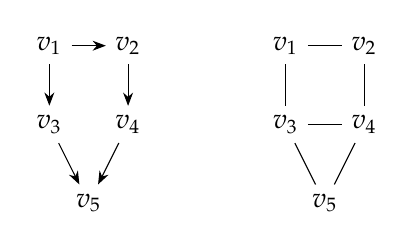
\begin{tikzpicture}
%\tikzstyle{place}=[circle,draw=blue!50,fill=blue!20,thick,inner sep=0pt,minimum size=6mm]
\begin{scope}
    \node (A) at (0,0) {$v_1$};
    \node (B) at (1,0) {$v_2$};
    \node (C) at (0,-1) {$v_3$};
    \node (D) at (1,-1) {$v_4$};
    \node (E) at (0.5,-2) {$v_5$};
    
    \node (F) at (3,0) {$v_1$};
    \node (G) at (4,0) {$v_2$};
    \node (H) at (3,-1) {$v_3$};
    \node (I) at (4,-1) {$v_4$};
    \node (J) at (3.5,-2) {$v_5$};
\end{scope}

\begin{scope}[>={Stealth[black]},
              every node/.style={fill=white,circle},
              every edge/.style={draw=black}]
    \path [->] (A) edge (B);
    \path [->] (A) edge (C);
    \path [->] (B) edge (D);
    \path [->] (C) edge (E);
    \path [->] (D) edge (E);
    
    \path [-] (F) edge (G);
    \path [-] (F) edge (H);
    \path [-] (G) edge (I);
    \path [-] (H) edge (I);
    \path [-] (H) edge (J);
    \path [-] (I) edge (J);
%    \path [-] (B) edge [bend right=60] (E); 
\end{scope}
\end{tikzpicture}
\caption{A DAG $G=(V,E)$ and its moral graph $H=(V,U(E)\cup F)$, in which $v_3v_4 \in F$ is a filled edge.}
\label{fg:envelope}
\end{figure}
\end{example}

If a given Bayesian network $<G=(V,E),\mathcal{P}>$ is faithful, the Markov blanket of a variable $u$ consists of its parents, children and children's other parents. For any spouse $v$ of $u$ that is neither a parent nor child of $u$, the edge $uv$ is a filled edge to make the moral graph $H$ of $G$. Hence, for each node $u \in V$, there is a one-to-one correspondance between its Markov blanket in $G$ and its neighbourhood in $H$. For example, in Figure \ref{fg:envelope} $B_G(v_3)=\{v_1,v_5,v_4\}=N_H(v_3)$.
\begin{definition}
\label{def:collider}
A \textbf{collider} in a hybrid graph is a node with at least two parents. 
\end{definition}

\begin{definition}
\label{def:consistent_ext}
A directed acyclic graph $G=(V,E)$ is a \textbf{consistent extension} of a hybrid graph $H=(V,F)$ if $U(E)=U(F)$ and $G$ and $H$ have the same set of colliders. 
\end{definition}

\begin{definition}
\label{def:subgraph}
Let $G'=(V',E')$ and $G=(V,E)$ be two graphs. If $V' \subseteq V$ and $E' \subseteq E$, then $G'$ is a \textbf{subgraph} of $G$, written as $G' \subseteq G$. 
\end{definition}

\begin{definition}
\label{def:induced_subgraph}
Let $G'=(V',E')$ and $G=(V,E)$ be two graphs. If $G'\subseteq G$ and $uv \in E$ for all $u,v \in V'$, then $G'$ is an \textbf{induced subgraph} of $G$, written as $G'=G[V']$.
\end{definition}
For simplicity, if $V' \subset V$ then we use $G-V'$ to denote $G[V\setminus V']$. If $V'=\{u\}$, then we use $G-u$. If $V'=V(H)$, then we use $G-H$. Similarly, if $E' \subset E$ then we use $G+E'$ and $G-E'$ to denote $(V,E \cup E')$  and $(V,E\setminus E')$ respectively. If $E' = \{uv\}$ then we use $G+uv$ or $G-uv$ instead.

\begin{definition}
Let $G=(V,E)$ be a graph. The set of \textbf{neighbours} of $u$ in $G$ is $N(u)=\{v \in V \mid uv \in E\}$. The closed neighbourhood of $u$ in $G$ is $N[u]=N(u)\cup \{u\}$.
\end{definition}
It is also useful to define the neighbours of a subgraph $H \subset G$ as $N_G(H)=\{u \in V\setminus V(H) \mid uv \in E, \forall v \in V(H)\}$.

\begin{definition}
Let $G=(V,E)$ be a graph. The \textbf{maximum degree} of the graph is $\Delta(G)=\max\{d(u) \mid u \in V\}$, where $d(u)=|N(u)|$ is the degree of $u$.
\end{definition}

\begin{definition}
A \textbf{clique} is a subset of nodes in a graph where every two distinct nodes are adjacent. 
\end{definition}

\begin{definition}
A \textbf{simplicial node} in a graph is a node whose neighbours form a clique. 
\end{definition}

\begin{definition}
Let $G=(V,E)$ be a graph. The \textbf{deficiency} of a node $x$ in $G$ is $D(x)=\{uv \notin E \mid u, v \in N(x)\}$.
\end{definition}
A node $u$ is simplicial in $G$ if and only if $D(u)=\emptyset$. That is, no edge needs to be filled in to make the neighbours of $u$ a clique. We write $D(G)\neq \emptyset$ if $D_G(u)\neq \emptyset, \forall u \in V$. And $D(G)=\emptyset$ if $\exists x \in V$ s.t. $D(x)=\emptyset$.
\begin{example}
In the moral graph $H$ as shown in Figure \ref{fg:envelope}, $D_H(v_1)=\{v_2v_3\}$ and $D_H(v_5)=\emptyset$. 
\end{example}

\begin{definition}
A \textbf{chord} in a m-cycle $C_m=v_1\dots v_mv_1$ is an edge $v_iv_j \notin E(C_m)$ for $i,j \in [1,m]$.
\end{definition}

\begin{definition}
A graph is \textbf{chordal} if each m-cycle for $m \ge 4$ has a chord.
\end{definition}

\begin{definition}
An \textbf{ordering} of a graph $G=(V,E)$ with $n$ vertices is a bijection $\alpha: \{1, \dots, n\} \leftrightarrow V$. 
\end{definition}
Another equivalent property as being chordal is that $G$ has a \textit{perfect elimination ordering}. That is, for each $x \in V$ with $\alpha^{-1}(x)=i+1$, we have $D_{G^i}(x)=\emptyset$, where $G^i=G-\{\alpha(1),\dots,\alpha(i)\}$ and $G^0=G$.

\begin{definition}
A graph $G=(V,E)$ is \textbf{recursively simplicial} if $\exists x \in V$ with $D_G(x)=\emptyset$ s.t. the induced subgraph $G-x$ is recursively simplicial. 
\end{definition}
Being recursively simplicial is equivalent as being chordal. It makes chordality a hereditary property. The following concept is not as strong as recursively simplicial, so it requires some edges to be removed in addition to the removal of a simplicial node. 

\begin{definition}
\label{def:wrs}
A graph $G=(V,E)$ is \textbf{weak recursively simplicial} if $\exists x \in V$ with $D_G(x)=\emptyset$ and $\exists E'\subseteq \{uv \in E \mid u,v \in N_G(x)\}$ s.t. the subgraph $G'=G-x-E'$ is weak recursively simplicial. 
\end{definition}

\begin{example}
\begin{figure}[H]
\centering
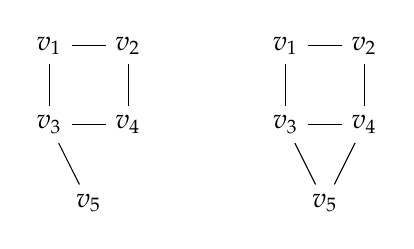
\begin{tikzpicture}
%\tikzstyle{place}=[circle,draw=blue!50,fill=blue!20,thick,inner sep=0pt,minimum size=6mm]
\begin{scope}
    \node (A) at (0,0) {$v_1$};
    \node (B) at (1,0) {$v_2$};
    \node (C) at (0,-1) {$v_3$};
    \node (D) at (1,-1) {$v_4$};
    \node (E) at (0.5,-2) {$v_5$};
    
    \node (F) at (3,0) {$v_1$};
    \node (G) at (4,0) {$v_2$};
    \node (H) at (3,-1) {$v_3$};
    \node (I) at (4,-1) {$v_4$};
    \node (J) at (3.5,-2) {$v_5$};
\end{scope}

\begin{scope}[>={Stealth[black]},
              every node/.style={fill=white,circle},
              every edge/.style={draw=black}]
    \path [-] (A) edge (B);
    \path [-] (A) edge (C);
    \path [-] (B) edge (D);
    \path [-] (C) edge (D);
    \path [-] (C) edge (E);
    
    \path [-] (F) edge (G);
    \path [-] (F) edge (H);
    \path [-] (G) edge (I);
    \path [-] (H) edge (I);
    \path [-] (H) edge (J);
    \path [-] (I) edge (J);
%    \path [-] (B) edge [bend right=60] (E); 
\end{scope}
\end{tikzpicture}
\caption{An example of a non-weak recursively simplicial graph $G$ (left) and a weak recursively simplicial graph $H$ (right).}
\label{fg:wrs}
\end{figure}

$H$ is a weak recursively simplicial (WRS) graph that can be justified by the following two criterion:
\begin{enumerate}
\item recursively removing $\{v_5, v_3v_4\}$, $\{v_3\}$, $\{v_4\}$, $\{v_1\}$, $\{v_2\}$ to eliminate the graph completely,
\item each node removed is a simplicial node in the current graph.
\end{enumerate}
On the other hand, the graph $G$ is not WRS, because there is no way $G$ can be eliminated completely whilst the node removed at each step is simplicial in the current graph. 
\end{example}

If a graph is recursively simplicial (i.e., chordal), it is also weak recursively simplicial with $E'=\emptyset$ for each simplicial node $x$. The converse, however, is not true. For example, the graph $H$ in Figure \ref{fg:wrs} is WRS but not chordal. 

\begin{definition}
A set of \textbf{excesses} of a graph $G=(V,E)$ according to an ordering $\alpha$ is a bijection $\epsilon_{\alpha}: \alpha \leftrightarrow \{\epsilon_{\alpha}(v_1), \dots, \epsilon_{\alpha}(v_n)\}$, where each $\epsilon_{\alpha}(v_i) \subseteq E(G[N(v_i)])$ consists of some edges between the neighbours of $v_i$.
\end{definition}
The composition $\kappa=(\alpha,\epsilon_{\alpha})$ of an ordering and a set of excesses is called an elimination kit of a graph $G$. We use $\kappa(1)$ to denote the node $\alpha(1)$ and its excess $\epsilon_{\alpha}(\alpha(1))$. By using the concept of elimination kit, we extend the definition of the subgraph $G^i=G-\{\kappa(1),\dots,\kappa(i)\} \subset G$ for $i\in [1,n]$, with the same convention $G^0=G$. 

\begin{example}
\label{ex:ek}
An ordering $\alpha=(v_5,v_3,v_4,v_1,v_2)$ and a set of excesses $\epsilon_{\alpha}=(\emptyset,\emptyset,\emptyset,\emptyset,\emptyset)$ form an elimination kit of $H$ in Figure \ref{fg:envelope}. 
\end{example}

\begin{definition}
Let $G=(V,E)$ be a graph and $\kappa=(\alpha, \epsilon_{\alpha})$ be an elimination kit of $G$. It is a \textbf{perfect elimination kit} if for each $x \in V$ with $\alpha^{-1}(x)=i+1$, we have $D_{G^{i}}(x)=\emptyset$.
\end{definition}
In general, a graph may have none, one or more than one perfect elimination kit (pek). 
\begin{example}
\label{ex:pek}
The elimination kit in Example \ref{ex:ek} is not perfect, because $D_{G^1}(v_3)\neq \emptyset$. The only pek for $H$ is $\alpha=(v_5,v_3,v_4,v_1,v_2)$ and $\epsilon_{\alpha}=(\{v_3v_4\},\emptyset,\emptyset,\emptyset,\emptyset)$. 
\end{example}

\begin{definition}
Let $G=(V,E)$ be a graph and $\kappa=(\alpha, \epsilon_{\alpha})$ be an elimination kit of $G$. It is a \textbf{partial perfect elimination kit} if there exists a non-empty subgraph $G^i \subset G$ s.t. $D(G^i)\neq \emptyset$ and $D_{G^{j-1}}(\alpha(j))=\emptyset$ for $j \in [1,i]$.
\end{definition}
A 4-cycle has no partial pek, because it has no simplicial node. A graph that has a pek may also has a partial pek.
\begin{example}
Example \ref{ex:ek} is a partial pek, because $D(G^1)\neq \emptyset$ and $D_{G^0}(v_5)=\emptyset$. 
\end{example}

\begin{definition}
A graph $H=(V,E\cup F)$ is called a \textbf{moralization} of an undirected graph $G=(V,E)$ if $H$ is moral. 
\end{definition}

Without loss of generality, assuming $F\neq \emptyset$ and $E\cap F=\emptyset$. Every edge $e\in E\cup F$ is either an edge of the underlying graph $G$ or a \textit{fill edge} in $F$. 

\begin{definition}
Let $G=(V,E)$ be a graph, and $H=(V,E\cup F)$ be a moral graph with $F\neq \emptyset$ and $E\cap F=\emptyset$. $H$ is a \textbf{minimal moralization} of $G$ if $(V,E\cup F')$ is non-moral $\forall F' \subsetneq F$. It is the \textbf{minimum moralization} if $\nexists E'$ with $|E'| < |F|$ s.t. the graph $(V,E\cup E')$ is moral. 
\end{definition}
Sometimes people also refer the set of fill edges $F$ as a minimal moralization instead of the graph $H$. The following is an  example of a minimal and minimum moralizations. 
\begin{figure}[H]
\centering
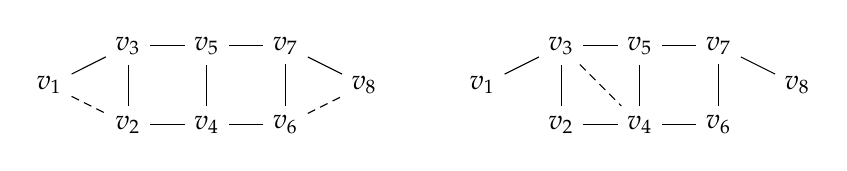
\begin{tikzpicture}
%\tikzstyle{place}=[circle,draw=blue!50,fill=blue!20,thick,inner sep=0pt,minimum size=6mm]
\begin{scope}         
    \node (a) at (-1,0.5) {$v_1$};
    \node (b) at (0,0) {$v_2$};   
    \node (c) at (0,1) {$v_3$};
    \node (d) at (1,0) {$v_4$};
    \node (e) at (1,1) {$v_5$};
    \node (f) at (2,0) {$v_6$};
    \node (g) at (2,1) {$v_7$};
    \node (h) at (3,0.5) {$v_8$};
            
    \path [-] (a) edge (c);
    \path [densely dashed] (a) edge (b);
    \path [-] (b) edge (c);
    \path [-] (b) edge (d);
    \path [-] (c) edge (e);
    \path [-] (d) edge (e);
    \path [-] (d) edge (f);
    \path [-] (e) edge (g);
    \path [-] (f) edge (g);
    \path [-] (g) edge (h);
    \path [densely dashed] (f) edge (h);
\end{scope}
\begin{scope}         
    \node (a) at (-1+5.5,0.5) {$v_1$};
    \node (b) at (0+5.5,0) {$v_2$};   
    \node (c) at (0+5.5,1) {$v_3$};
    \node (d) at (1+5.5,0) {$v_4$};
    \node (e) at (1+5.5,1) {$v_5$};
    \node (f) at (2+5.5,0) {$v_6$};
    \node (g) at (2+5.5,1) {$v_7$};
    \node (h) at (3+5.5,0.5) {$v_8$};
            
    \path [-] (a) edge (c);
    \path [densely dashed] (c) edge (d);
    \path [-] (b) edge (c);
    \path [-] (b) edge (d);
    \path [-] (c) edge (e);
    \path [-] (d) edge (e);
    \path [-] (d) edge (f);
    \path [-] (e) edge (g);
    \path [-] (f) edge (g);
    \path [-] (g) edge (h);
\end{scope}
\end{tikzpicture}
\caption{An example of a minimal (left) and minimum (right) moralizations.}
\label{fg:mini_moral}
\end{figure}

\begin{definition}
Let $\kappa=(\alpha,\epsilon_{\alpha})$ be an elimination kit of a graph $G$. $\kappa$ is \textbf{minimal} if there is no other elimination kit $\kappa'$ s.t. $G_{\kappa'}^+$ is a proper subgraph of $G_{\kappa}^+$. It is \textbf{perfect} if $G_{\kappa}^+=G$. 
\end{definition}

\begin{definition}
Let $G=(V,E)$ be a connected graph. A vertex set $S\subset V$ is a \textbf{separator} if $G[V-S]$ is disconnected. 
\end{definition}

\begin{definition}
A graph $G$ is called \textbf{connected} if there is a path between every pair of vertices in $G$. 
\end{definition}

\begin{definition}
Let $G$ be a graph. A maximal connected subgraph of $G$ is called a \textbf{component} of $G$. 
\end{definition}

\begin{definition}
Given two non-adjacent vertices $u,v$ in a graph $G=(V,E)$. A vertext set $S \subset V$ is a \textbf{$u,v$-separator} if $u$ and $v$ belong to different components of $G[V-S]$. In particular, $S$ is a \textbf{minimal} $u,v$-separator if there exists no proper subset of $S$ that separates $u$ and $v$. 
\end{definition}


\section{Minimal moralization}
From now on, we try to develop polynomial time algorithms for finding the maximal moral subgraph or the minimal moral supergraph of a given non-moral graph $F$.

\begin{definition}
A \textbf{simple cycle} $C$ in a graph is a closed walk such that each node in $V(C)$ is only visited once except for the starting node.
\end{definition}

\begin{definition}
An \textbf{induced simple cycle} in a graph $F$ is a simple cycle that is an induced subgraph of $F$. 
\end{definition}

\begin{remark}
The number of induced simple cycles of length 4 or more in $F$ gives an upper bound of the number of edges to be added/removed from $F$.
\end{remark}

\begin{remark}
The minimal moral supergraph problem is NP-complete, because if it is polynomial then we can run an algorithm to find the minimal moral supergraph of a graph $F$ and comparing it with $F$. This will identify if $F$ is moral or not in polynomial time. 
\end{remark}

Both minimum triangulation and maximum chordal subgraph seem to be only solvable in NP-complete time complexity. But minimal triangulation and maximal subgraphs seem to be solvable in efficient time. 

Minimal triangulation is related to minimal separator. A vertext $S\subset V$ is a \textbf{separator} if $F[V\setminus S]$ is disconnected. Given two vertices $u,v\in V$, $S$ is a $u,v$-separator if $u$ and $v$ belong to different connected components of $F[V\setminus S]$. $S$ is called a minimal $u,v$-separator if $S$ has no proper subset that separates $u$ and $v$. A vertex $S\subset V$ is a \textbf{minimal separator} of $F=(V,E)$ if $\exists u, v \in V$ s.t. $S$ is a minimal $u,v$-separator. 
 

\begin{itemize}
\item Chordality is not preserved under graph complementation, so finding the maximal chordal subgraph is not reducible to finding minimal chordal supergraphs. This is the same for morality, I've just randomly generated some graphs and their complements, they nont always have the same morality. 
\item Chordality is a hereditary property. That is, if a graph $F=(V,E)$ is chordal, the subgraph of $F$ induced by $V\setminus \{x\}$ is also chordal where $x$ is a simplicial node in $F$. But morality is not a hereditary property, because the induced subgraph after removing a simplicial node from $F$ may or may not be moral. 
\item Since checking morality in general is NP-complete, I suspect that the finding the minimal triangulation of a graph is al NP-complete. For otherwise, we could find the minimal triangulation of a graph and compare it with the original graph. If they are identical, then the original graph is NP-complete. 
\item Run backtracking algorithm on a graph, if the algorithm stucks, add pick a node with the minimum degree and add its deficiency. This way will result a graph that is moral (and perhaps chordal), but won't be a minimal moral supergraph. A moral graph is a minimal supergraph of a graph $F$ if there is no another moral graph that is a proper subgraph of it. 
\item Different ordering will result in different moral supergraph, hence the choice of a node to eliminate at each step is crucial. 
\end{itemize}


\subsection{Characterizations of minimal moralization}
Firstly, we prove that for each minimal moralization $H$ of $G$, there exists a mek $\kappa$ s.t. $H=G_{\kappa}^+$. The consequence of this result is that finding a minimal moralization or a mek are equivalent problems. The result is proved by the same logic as in \cite{ohtsuki1976minimal} for chordal graphs. 
\begin{lemma}
\label{lm:ohtsuki_lm1}
Let $G=(V,E)$ be a graph and $H=(V,E\cup F)$ be a minimal moralization of $G$. Then there exists a minimal elimination kit $\kappa$ s.t. $G_{\kappa}^+=H$. 
\end{lemma}
\begin{proof}
$H$ is moral implies it has a pek $\kappa$. $G \subset H$ implies $G_{\kappa}^+=(V,E\cup F') \subset H$. Since $H$ is minimal, $F'=F$ and consequently $G_{\kappa}^+=H$. Assuming $H$ has another pek $\kappa'$ with $G_{\kappa'}^+ =(V,E\cup E') \subsetneq G_{\kappa}^+$. It entails that $E' \subsetneq F$, which contradicts $H$ being minimal. \qed
\end{proof}

\begin{lemma}
\label{lm:ohtsuki_lm2}
Let $\kappa$ be a minimal elimination kit of a graph $G=(V,E)$. Then $G_{\kappa}^+$ is a minimal moralization of $G$. 
\end{lemma}
\begin{proof}
Assuming $G_{\kappa}^+=(V,E\cup E')$ is not minimal. That is, there exists another set of fill edges $F\subsetneq E'$ with $H=(V,E\cup F)$ being moral. Without loss of generality, assuming $H$ is a minimal. Lemma \ref{lm:ohtsuki_lm1} implies that $\exists \kappa'$ s.t. $G_{\kappa'}^+=H \subsetneq G_{\kappa}^+$. It contradicts with $\kappa$ being a mek. \qed
\end{proof}

\begin{theorem}
\label{thm:ohtsuki_thm1}
A graph $H$ is a minimal moralization of $G$ if and only if there exists a minimal elimination kit $\kappa$ s.t. $H=G_{\kappa}^+$.
\end{theorem}
\begin{proof}
The theorem follow from Lemma \ref{lm:ohtsuki_lm1} and Lemma \ref{lm:ohtsuki_lm2}. \qed 
\end{proof}

\begin{theorem}
A graph is moral if and only if it has a perfect elimination kit. 
\end{theorem}
\begin{proof}
The proof is trivial. \qed
\end{proof}

If there exists a perfect elimination kit (pek) $\kappa$ with $\epsilon_{\alpha} =\emptyset$, then $G$ is chordal and the outputs $G_{\kappa}^+=G_{\alpha}^+$. 

The EA algorithm outputs a moralized graph that possibly contains more edges than needed for moralization. To pursue a smaller moralized graph, the \textit{minimal moralization sandwich problem} looks for a minimal moralization $H$ of $G$ s.t. $G \subseteq H \subseteq G_{\kappa}^+$ for a given elimination kit. 

The following lemmas and theorems are stated and proved in similar ways as those for triangulated graphs in \cite{rose1976algorithmic}. 

\begin{lemma}
\label{lm:rose_lm1}
Let $G=(V,E)$ be a moral graph with a pek $\kappa=(\alpha,\epsilon_{\alpha})$. For any node $x \in V$, the graph $G'=(V,E\cup D_G(x))$ has a pek $\kappa'=(\alpha, \epsilon'_{\alpha})$. 
\end{lemma}  
\begin{proof}
We want to show that for any two distinct edges $\{v_iv_j, v_iv_k\} \subset E\cup D_G(x)-E'$ with $\alpha^{-1}(v_i) < \min \{\alpha^{-1}(v_j), \alpha^{-1}(v_k)\}$, the edge $v_jv_k \in E\cup D_G(x)-E'$ where $E' = \{\epsilon'_{\alpha}(v_1),\dots,\epsilon'_{\alpha}(v_{i-1})\}$ is the set of removed edges up to $v_i$ according to $\kappa'$.

\textit{Case 1:} If $\{v_iv_j, v_iv_k\} \subset E-E'$, since $v_i$ comes before $v_j$ and $v_k$ in $\alpha$, the edge $v_jv_k\in E-E'$ because $\kappa'$ is perfect.

\textit{Case 2:} If $\{v_iv_j, v_iv_k\} \subset D_G(x)-E'$, then $\{v_i,v_j,v_k\} \subset N_G(x)$ so $v_jv_k \in D_G(x)$. It remains to show that $v_jv_k \notin E'$. If there is a node $v_l$ with $\alpha^{-1}(v_l) < \alpha^{-1}(v_i)$ and $v_jv_k\in \epsilon_{\alpha}(v_l)$ because it is in a cycle, then it is possible for $v_jv_k \in \epsilon'_{\alpha}(v_i)$ to break the same cycle. 
\begin{figure}[H]
\centering
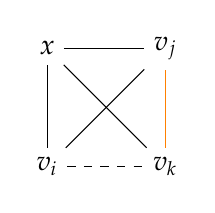
\begin{tikzpicture}
%\tikzstyle{place}=[circle,draw=blue!50,fill=blue!20,thick,inner sep=0pt,minimum size=6mm]
\begin{scope}         
    \node (a) at (0,0) {$v_i$};
    \node (b) at (0,1.5) {$x$};   
    \node (c) at (1.5,0) {$v_k$};
    \node (d) at (1.5,1.5) {$v_j$};
            
    \path [-] (a) edge (b);
    \path [dashed] (a) edge (c);
    \path [-] (a) edge (d);
    \path [-] (b) edge (c);
    \path [-] (b) edge (d);
    \path [-][orange] (c) edge (d);
\end{scope}
\end{tikzpicture}
\caption{An example of case 3. The solid lines are in $E$. The dashed is in $D(x)$. The orange is the edge we want to prove to belong to $E\cup D(x)$.}
\label{fg:case3}
\end{figure}
\textit{Case 3:} If $v_iv_j \in E-E'$ and $v_iv_k \in D_G(x)-E'$, then $\{v_i,v_k\}\subset N_G(x)$. If $x=v_j$ then $v_jv_k \in E$. Otherwise (Figure \ref{fg:case3}), we have $\alpha^{-1}(v_i) < \alpha^{-1}(x)$ because $v_iv_k \in D_G(x)$. If so, $xv_j \in E$ because $\{x, v_j\} \subset N_G(v_i)$. It then follows that $v_jv_k \in E\cup D_G(x)$ because $\{v_j,v_k\} \subset N_G(x)$. For the same argument in case 2, $v_jv_k \notin E'$. \qed
\end{proof}

\begin{corollary} 
\label{cor:rose_cor2}
Let $G=(V,E)$ be a moral graph and $x$ be any node with $D_G(x)=\emptyset$. Then there is a pek $\kappa=(\alpha,\epsilon_{\alpha})$ of $G$ with $\alpha(1) = x$.
\end{corollary}
\begin{proof}
Let $R=\{x \mid D_G(x)=\emptyset\}$. Morality implies that $|R|\ge 1$. If $|R|=1$, it is certain that $\alpha(1)=x$. Otherwise, for any $x\in R$, there is a different pek $\kappa=(\alpha,\epsilon_{\alpha})$ for $G$ with $\alpha(1)=x$.  \textcolor{red}{Not quite a proof!} \qed
\end{proof}

\begin{corollary}
\label{cor:rose_cor1}
Let $G=(V,E)$ be a moral graph with a pek $(\alpha, \epsilon_{\alpha})$ and $x$ is any node in $G$. Then there exists a pek $\kappa'=(\alpha,\epsilon'_{\alpha})$ for the graph $G'=(V,E\cup D_G(x))$ s.t. the subgraph $G'_x = (V-\{x\},E(G[V\setminus \{x\}])\cup D_G(x)-\epsilon'_{\alpha}(x))$ is also moral. 
\end{corollary}
\begin{proof}
Lemma \ref{lm:rose_lm1} implies that $G'=(V,E\cup D_G(x))$ is moral. Corollary \ref{cor:rose_cor2} suggests that $G'$ has a pek $\kappa'=(\alpha,\epsilon'_{\alpha})$ with $\alpha(1)=x$. Hence, $G'_x = (V-\{x\},E(G[V\setminus \{x\}])\cup D_G(x)-\epsilon'_{\alpha}(x))$ is also moral because of the hereditary property of morality. \qed
\end{proof}

\begin{lemma}
\label{lm:rose_lm2}
Let $G=(V,E)$ and $H=(V,E\cup F)$ be moral graphs with peks $(\alpha,\epsilon_{\alpha})$ and $(\beta,\epsilon_{\beta})$ respectively and $F\neq \emptyset$, $E \cap F=\emptyset$. Then there exists at least one edge $f=uv \in F$ with $\beta^{-1}(u) < \beta^{-1}(v)$ s.t. $H-f-E'=(V,E\cup F-\{f\}-E')$ is moral, where $E'=\{vw \in F \mid vw \in \epsilon_{\beta}(u)\}$.
\end{lemma}
\begin{proof}
We prove the lemma by induction on the number of nodes. When $|V| \le 3$, all graphs are moral so the lemma is true. Assuming it is true for $|V|=n-1 \ge 4$, we want to show that the lemma is also true for $n$ nodes. Let $R=\{x\mid D_G(x)=\emptyset\}$ and $S=\{x\mid D_{H}(x)=\emptyset\}$. Since both graphs are moral, none of these sets is empty. The proof is divided into two cases, depending on whether or not there exists a node $u \in S$ with $f=uv \in F$.

\textit{Case 1:} $\exists u \in S$ with  $f=uv\in F$. Since $u\in S$, Corollary \ref{cor:rose_cor2} suggests $H$ has a pek $(\beta,\epsilon_{\beta})$ with $\beta(1)=u$. Furthermore, $N_H(u)-\{v\}$ still forms a clique after removing $f$ and $E'$ that contains the edges between $v$ and the other neighbours of $u$. Therefore, $H-f-E'$ is moral with a pek $(\beta,\epsilon_{\beta}-E')$. 

\textit{Case 2:} $\nexists u \in S$ with  $f=uv\in F$. In this case, we want to show that $\exists x\in S$ with $F\nsubseteq D_G(x)$. (\textcolor{red}{an exmaple is sufficient}?) Assuming $\nexists x \in S$. That is, $\forall x\in S$ satisfy $F\subseteq D_G(x)$. Being in $S$ implies $D_G(x) \subseteq F$, so $F=D_G(x)$. For any node $x\in R$, Corollary \ref{cor:rose_cor2} suggests there is a pek $(\alpha, \epsilon_{\alpha})$ for $G$ with $\alpha(1)=x$. Lemma \ref{lm:rose_lm1} implies $(\alpha,\epsilon'_{\alpha})$ is a pek for $(V,E\cup D(x))=(V,E\cup F)=H$, hence $x\in S$. Therefore, for any node in $R$, it is also in $S$. But $x\in R$ implies $D_G(x)=\emptyset$. In conjunction with $F\neq \emptyset$, it entails that $F \nsubseteq D_G(x)$ that is a contradiction. Therefore, if case 2 is true $\exists x\in S$ with $F\nsubseteq D_G(x)$ (Figre \ref{fg:case2}). 
\begin{figure}[H]
\centering
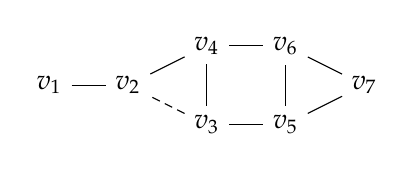
\begin{tikzpicture}
%\tikzstyle{place}=[circle,draw=blue!50,fill=blue!20,thick,inner sep=0pt,minimum size=6mm]
\begin{scope}          
    \node (a) at (-1,0.5) {$v_1$};
    \node (b) at (0,0.5) {$v_2$};   
    \node (c) at (1,0) {$v_3$};
    \node (d) at (1,1) {$v_4$};
    \node (e) at (2,0) {$v_5$};
    \node (f) at (2,1) {$v_6$};    
   	\node (g) at (3,0.5) {$v_7$};
            
    \path [-] (a) edge (b);
    \path [densely dashed] (c) edge (b);
    \path [-] (c) edge (d);
    \path [-] (d) edge (b);
    \path [-] (c) edge (e);
    \path [-] (d) edge (f);
    \path [-] (e) edge (f);
    \path [-] (e) edge (g);
    \path [-] (f) edge (g);
\end{scope}
\end{tikzpicture}
\caption{An example of case 2, where $F=\{v_2v_3\}$, $R=S=\{v_1,v_7\}$. Each node $x\in S$ satisfies that $F\nsubseteq D_G(x)$.}
\label{fg:case2}
\end{figure}
For such a node $x \in S$, Lemma \ref{lm:rose_lm1} and Corollary \ref{cor:rose_cor1} imply the following moral graphs and peks
\begin{align*}
G &= (V,E) \text{ with } (\alpha,\epsilon_{\alpha}) \\
G' &=(V,E\cup D_G(x)) \text{ with } (\alpha, \epsilon'_{\alpha}) \\
G'_x&=(V-\{x\}, E(G[V-\{x\}])\cup D_G(x)-\epsilon'_{\alpha}(x))\\
H &= (V,E\cup F) \text{ with } (\beta, \epsilon_{\beta}) \\
H' &=(V,E\cup F \cup D_G(x)) \text{ with } (\beta, \epsilon'_{\beta})\\
H'_x&=(V-\{x\}, E(G[V-\{x\}])\cup F\cup D_G(x)-\epsilon'_{\beta}(x)).
\end{align*}
$F\nsubseteq D(x)$ entails $G' \subsetneq H'$. Since $\alpha(1)=\beta(1)=x$, there exist excesses s.t. $\epsilon'_{\beta}(x) \subseteq \epsilon'_{\alpha}(x)$. Let $F'=E(H'_x)-E(G'_x)=(F-D(x))\cup (\epsilon'_{\alpha}(x)-\epsilon'_{\beta}(x))$. It follows that $F'\neq \emptyset$ and $F' \cap E(G'_x)=\emptyset$. By the inductive hypothesis, there exists an edge $f=uv \in F'$ with $\beta^{-1}(u)<\beta^{-1}(v)$ s.t. $H'_x-f-E'$ is moral where $E'=\{vw \in F' \mid vw \in \epsilon'_{\beta}(u)\}$. Neither of $\{f\}$ or $E'$ is in $D(x)$, so adding $\{x\}$ and $\epsilon'_{\beta}(x)$ back to $H'_x$ does not change the morality of $H'-f-E'$. \qed
\end{proof}

The following theorem is one of the main results for this section. 
\begin{theorem}
Let $G=(V,E)$ be a graph, and $G'=(V,E\cup F)$ be a moralization of $G$ with $E\cap F=\emptyset$. Then $F$ is a minimal moralization if and only if there exists a pek $(\beta,\epsilon_{\beta})$ s.t. for each $f=uv \in F$ with $\beta^{-1}(u) < \beta^{-1}(v)$, $G'-f-E'=(V,E\cup F -\{f\}-E')$ is not moral, where $E'=\{vw \in F \mid vw \in \epsilon_{\beta}(u)\}$.
\end{theorem}
\begin{proof}
The theorem is proved by the definition of minimal moralization and Lemma \ref{lm:rose_lm2}. \qed 
\end{proof}
A consequence of the theorem is that if both $F$ and $H$ are moralizations of $G$ and $F \subsetneq H$, then there is a sequence of subsets of edges $\{f\}\cup E'$ that can be removed from $H$ one by one, such that the resulting graph after each removal is moral. 

Every minimal separater of a chordal graph is a clique \cite{dirac1961rigid}. This result, however, is not true for moral graphs which are more general than chordal graphs. The following theorem states the relation between minimal separater and moral graphs. 
\begin{theorem}
A graph $G=(V,E)$ is moral if and only if there exists an elimination kit $\kappa=(\alpha,\epsilon_{\alpha})$ s.t. for every pair of non-adjacent vertices $u,v\in V$ with $i=\min\{\alpha^{-1}(u),\alpha^{-1}(v)\}$, the minimal $u,v$-separator is a clique in $G^i=G-\{\alpha(1),\dots,\alpha(i-1)\}-\{\epsilon_{\alpha}(\alpha(1)),\dots,\epsilon_{\alpha}(\alpha(i-1))\}$.
\end{theorem}
\begin{proof}
If $G$ is moral with $n$ nodes, there exists a pek $\kappa=(\alpha, \epsilon_{\alpha})$. Without loss of generality, assuming $i=\alpha^{-1}(u) < \alpha^{-1}(v)$ for any two nodes $u,v \in V$. In addition, $uv \notin E$ implies that $v$ is separated from $u$ by $S\subseteq N_G(u)$. Since $\kappa$ is a pek, $u$ must be a simplicial node in the subgraph $G^i$. Therefore, $N_G(u)$ forms a clique and consequently any subset of it is also a clique. 

To prove the sufficient condition, assume $G$ is not moral. That is, $\exists H \subset G$ a mpe subgraph s.t. $D(H)\neq \emptyset$. Hence, $\exists C_m \subset H$ an atomic cycle for $m \ge 4$ st. $\exists u,v \in V(C_m)$ with $uv \notin E(C_m)$. Therefore, the minimal $u,v$-separator is not a clique, which is a contradiction. \qed
\end{proof}


\subsection{Minimal moralization algorithms}
We have defined $G^i=G-\{\alpha(1),\dots,\alpha(i-1)\}-\{\epsilon_{\alpha}(\alpha(1)),\dots,\epsilon_{\alpha}(\alpha(i-1))\}$, which can be interpreted as the resulting graph in step $i$ of the EG algorithm. 
\begin{definition}
Let $G=(V,E)$ be a graph and $\kappa=(\alpha,\epsilon_{\alpha})$ be an eliminiation kit of $G$. If $D_{G^i}(\alpha(i))=\emptyset$ for $i \in [1,p]$ and $\nexists \kappa'=(\beta,\epsilon_{\beta})$ s.t. $D_{G^i}(\beta(i))=\emptyset$ for $i \in [1,q]$ and $\{\alpha(1),\dots,\alpha(p)\}\subsetneq \{\beta(1),\dots,\beta(q)\}$ where $p,q \le |V|$, then $\kappa$ is called a \textbf{maximal perfect elimination kit} of $G$.
\end{definition}
If $\kappa$ is a maximal perfect elimination kit of $G$ with $D_{G^i}(\alpha(i))=\emptyset$ for $i \in [1,p]$, then $H=G-\{\alpha(1),\dots,\alpha(p)\}-\{\epsilon_{\alpha}(\alpha(1)),\dots,\epsilon_{\alpha}(\alpha(p))\}$ is called a \textit{minimal perfect eliminated (mpe) subgraph} of $G$. If $\kappa$ is a pek, then the mpe subgraph of $G$ is empty. If $D(G)\neq \emptyset$, then $G$ is the mpe subgraph of itself. 

\textbf{Conjecture:} If $H\subset G$ is a mpe subgraph of $G$, then a minimal moralization of $H$ is also a minimal moralization of $G$. If $G$ has many mpe subgraphs and none of them is overlapped, then this seems trivial. But if $\exists H_1,H_2\subset G$ are both mpe of $G$ and $H_1\cap H_2 \neq \emptyset$ then ?

\newpage
\section{Some random notes}
\begin{proposition}
Let $F$ be a moral 
\end{proposition}

\begin{figure}[H]
\centering
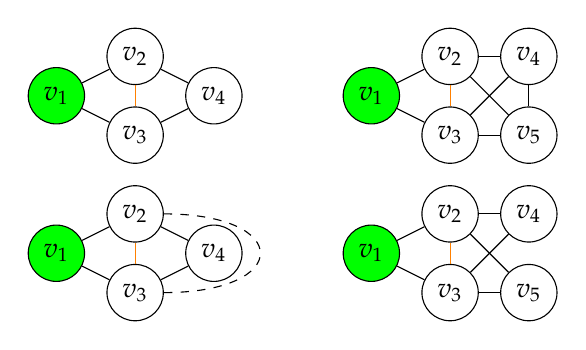
\begin{tikzpicture}
\begin{scope}[every node/.style={circle,draw}]               
	%k3+k3    
    \node[fill=green] (a) at (0,1) {$v_1$};
 	\node (b) at (1,1.5) {$v_2$};
 	\node (c) at (1,0.5) {$v_3$};
 	\node (d) at (2,1) {$v_4$};
    \path [-] (a) edge (b);
    \path [-] (a) edge (c);
    \draw[orange] (c) -- (b);        
    \path [-] (c) edge (d);
    \path [-] (b) edge (d);
    %k3+k4
    \node[fill=green] (aa) at (4,1) {$v_1$};
 	\node (bb) at (5,1.5) {$v_2$};
 	\node (cc) at (5,0.5) {$v_3$};
 	\node (dd) at (6,1.5) {$v_4$};
 	\node (ee) at (6, 0.5) {$v_5$};
    \path [-] (aa) edge (bb);
    \path [-] (aa) edge (cc);
    \draw[orange] (cc) -- (bb);        
    \path [-] (bb) edge (dd);
    \path [-] (cc) edge (ee);
    \path [-] (dd) edge (ee);
    \path [-] (dd) edge (cc);
    \path [-] (bb) edge (ee);   
    %k3+(k3+cm)
    \node[fill=green] (A) at (0,-1) {$v_1$};
 	\node (B) at (1,-0.5) {$v_2$};
 	\node (C) at (1,-1.5) {$v_3$};
 	\node (D) at (2,-1) {$v_4$};
    \path [-] (A) edge (B);
    \path [-] (A) edge (C);
    \draw[orange] (C) -- (B);     
    \path [-] (C) edge (D);
    \path [-] (B) edge (D);
    %k3+(k3+k3)
    \node[fill=green] (AA) at (4,-1) {$v_1$};
 	\node (BB) at (5,-0.5) {$v_2$};
 	\node (CC) at (5,-1.5) {$v_3$};
 	\node (DD) at (6,-0.5) {$v_4$};
 	\node (EE) at (6,-1.5) {$v_5$};
    \path [-] (AA) edge (BB);
    \path [-] (AA) edge (CC);
    \draw[orange] (CC) -- (BB);        
    \path [-] (CC) edge (DD);
    \path [-] (BB) edge (DD);
    \path [-] (BB) edge (EE);
    \path [-] (CC) edge (EE);        
    
\end{scope}
	\draw[dashed] (B) .. controls (3,-0.5) and (3,-1.5) .. (C);
\end{tikzpicture}
\caption{A simplicial $K_3$ over $\{v_1,v_2,v_3\}$ shares an edge with a $K_3$ (top left), $K_4$ (top right), $\{K_3, C_m\}$ (bottom left) or $\{K_3,K_3\}$ (bottom right).}
\label{fg:k3+}
\end{figure} 

\textbf{Lloyd's conjecture:} knowing a graph is WRS, adding an edge to obtain a supergraph, perhaps it is efficient to check if the supergraph is wrs.

\begin{proof}
because remove the added edge, then we obtain the original graph which we know is wrs. however, we don't remove a random edge when checking wrs unless the edge connects to a simplicial node. what if the edge is not connected with a sim node? if we know the original graph is wrs and we know the set of sim nodes in the recursion and the set of edges to delete, then we could easily check if the new edge is connected with any one of the sim node, if it is then good. if not, then we could check if the new edge is connected with two neighbours of a sim node, if it is then good. if a graph is wrs, then it eventually will diminish, so the new edge must appear somewhere in the recursion to either stop the recursion or don't stop it.
\end{proof} 

\begin{corollary}
DAGs in the same Markov equivalent class produce the same Markov blanket sets $B_X$. 
\end{corollary}
\begin{proof}
If two DAGs $G_1$ and $G_2$ are Markov equivalent, they have the same skeleton and the same set of colliders. This implies $B_i^{G_1} = B_i^{G_2}, \forall X_i \in X$. \qed
\end{proof}
Notice that two Markov equivalent classes could entail the same $B_X$. For example... 

\begin{corollary}
$|\{\text{chordal graphs}\}| \le |B_X| \le |\{\text{Markov equivalent classes}\}|$.
\end{corollary} 

Counting labelled chordal graphs \cite{wormald1985counting}, counting Markov equivalent classes (assymptotic ratio of around 0.27 to DAGs) \cite{gillispie2001enumerating}. 

\begin{table}[]
\centering
\caption{Comparison between the number of labelled connected chordal graphs, the number of weak recursively simplicial graphs, the number of undirected graphs and the number of Markov equivalent classes.}
\label{my-label}
\begin{tabular}{llllll}
\# nodes & \# con-C.G. & \# C.G. & \# WRS & \# U.G. & \# MEC \\ \hline
1        & 1& 1                 & 1          & 1         & 1 \\
2        & 1 & 2                 & 2          & 2         & 2 \\
3        & 4 & 8                 & 8          & 8         & 11 \\
4        & 35 & 61                & 61         & 64         & 185 \\
5        & 541 & 822               & 882        & 1024            & 8782\\
6        & 13302 & 18154             &       & 32768              & 1067825\\
7        & 489287 & 617675            &            & 2097152         & 312510571\\
8        & 25864897 & 30888596          &            &  268435456        & 212133402500 \\
9        & 1910753782 & 2192816760        &            &  68719476736       & 326266056291213 \\ 
10       & $1.93 \times 10^{11}$ & $2.15 \times 10^{11}$     &            & $3.52 \times 10^{13}$  & $1.19\times 10^{17}$ \\ \hline
\end{tabular}
\end{table}

\begin{proposition}
\label{prop:leaf_is_sim}
Let $G$ be a DAG and $F$ be the moral graph of $G$. If a node $x$ is a leaf in $G$, then it must be a simplicial node in $F$. 
\end{proposition}
\begin{proof}
If $x$ is a leaf in $G$, it has only parents, which form a clique after moralization. By definition, $x$ is a simplicial node in $F$. \qed
\end{proof}

\begin{corollary}
Let $G$ be a DAG and $F$ be the moral graph of $G$. Then $F$ must have at least one simplicial node. 
\end{corollary}

\begin{proof}
Since each DAG has at least one leaf, by Proposition \ref{prop:leaf_is_sim} $F$ have at least one simplicial node. \qed
\end{proof}

\begin{corollary}
\label{cor:negation_of_leaf_is_sim}
Let $G$ be a DAG and $F$ be the moral graph of $G$. If a node $x$ is not a simplicial node in $F$, then it must not be a leaf in $G$. 
\end{corollary}

\begin{proposition}
Let $G$ be a DAG and $F$ be the moral graph of $G$. Let $S^1$ be the set of simplicial nodes in $F$ and $F_1$ be the induced subgraph of $F$ over $X\setminus S^1$. Then there must exist at least one simplicial node after removing from $F'$ all the edges between $N(X_i), \forall X_i \in S^1$.
\end{proposition}

\begin{proof}
Let $F_1'$ be the result of removing from $F_1$ all the edges between $N(X_i), \forall X_i \in S^1$. The corresponding directed graph $G'$ of $F_1'$ must be a subgraph of the DAG $G$, so also acyclic. Assuming $F_1'$ has no simplicial nodes, by Corollary \ref{cor:negation_of_leaf_is_sim} $G'$ has no leaf, which is a contradiction. \qed
\end{proof}


Here are some issues worth discussing:
\begin{enumerate}
\item Application: the backtracking algorithm can now be applied when learning MBs in paralle. What if there are conflicts between two MBs, which one should give up? Need to estimate uncertainty?
\item Simplicial nodes in the first step always contain the leaves.
\item Those nodes that become simplicial in the next step without having to delete any edges contain the leaves in the next step. 
\item So wrs can be used to test if a MB family is consistent with a DAG, it would be good if we can also find out how many consistent DAGs or essential graphs are there for this MB family. 
\item also it would be good if we can explore wrs into details, such as what dag nodes become simplicial nodes in wrs recursion, and if no edges need to be deleted from a simplicial node's neighbours then what's this simplicial node?
\item maybe there is a path from s.t. every step is a moral graph of a dag, perhaps can be proved by delete an edge from a dag.   
\end{enumerate}

\textbf{Questions:} If a graph $F$ is known to be wrs, does is help to decide if a subgraph/supergraph different by one edge from $F$ is wrs or not?

\textbf{Answer:} Probably not. If it is, then we know a base case, any graph can be reached from this base case, hence any graph can be efficiently tested. 

\iffalse
The undirected edge connects two parents of a common child is called a \textit{moralized edge}. The process of obtaining a moral graph from a DAG is called \textit{moralization}. There is a unique moral graph of each DAG. Next, we define the reverse of a moralization process as \textit{demoralization}. It is defined on undirected graphs with at least one simplicial node. 
\fi

% the next proposition may not be true, so we omit it.
\iffalse
The next proposition proves that a chordal graph is also D-WRS, but not vice versa. 
\begin{proposition}
\label{prop:chordal_is_dwrs}
If $F=(V,E)$ is a chordal graph, then it is D-WRS. 
\end{proposition}
\begin{proof}
Assuming $F$ is not D-WRS. Then there is a subgraph $F' \subset F$ obtained by recursively remvoing all simplicial cliques from $F$ s.t. $F'$ has no simplicial clique. Hence, $F'$ must be cyclic 
\end{proof}


\begin{proof}
Being chordal is equivalent as being triangulated. If $F$ is chordal (Figure \ref{fg:chordal_is_dwrs}), removing the maximal simplicial clique of size 3 results in a subgraph of $F$ that has a maximal simplicial clique of size 2. Removing the size 2 maximal simplicial clique, we obtain a subgraph  that could also be obtained by recursively simplicial. \qed
\end{proof}
\begin{figure}[H]
\centering
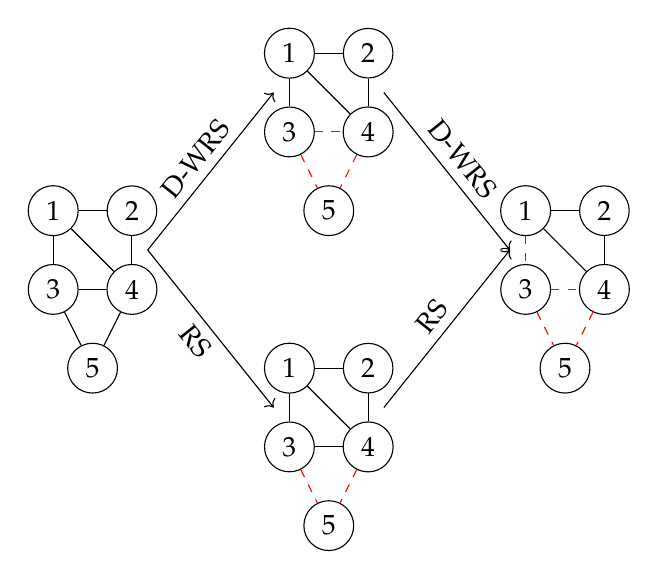
\begin{tikzpicture}
%\tikzstyle{place}=[circle,draw=blue!50,fill=blue!20,thick,inner sep=0pt,minimum size=6mm]
\begin{scope}[every node/.style={circle,draw}]  
    \node (F) at (0,0) {$1$};
    \node (G) at (1,0) {$2$};
    \node (H) at (0,-1) {$3$};
    \node (I) at (1,-1) {$4$};
    \node (J) at (0.5,-2) {$5$};
     
    \node (A) at (3,2) {$1$};
    \node (B) at (4,2) {$2$};
    \node (C) at (3,1) {$3$};
    \node (D) at (4,1) {$4$};
    \node (E) at (3.5,0) {$5$};
    
    \node (a) at (3,-2) {$1$};
    \node (b) at (4,-2) {$2$};
    \node (c) at (3,-3) {$3$};
    \node (d) at (4,-3) {$4$};
    \node (e) at (3.5,-4) {$5$};
    
    \node (K) at (6,0) {$1$};
    \node (L) at (7,0) {$2$};
    \node (M) at (6,-1) {$3$};
    \node (N) at (7,-1) {$4$};
    \node (O) at (6.5,-2) {$5$};
\end{scope}

\begin{scope}[>={Stealth[black]}]    
    \path [-] (F) edge (G);
    \path [-] (F) edge (H);
    \path [-] (G) edge (I);
    \path [-] (H) edge (I);
    \path [-] (H) edge (J);
    \path [-] (I) edge (J);
    \path [-] (F) edge (I);
        
    \path [-] (A) edge (B);
    \path [-] (A) edge (C);
    \path [-] (B) edge (D);
    \path [color=red,dashed] [-] (C) edge (D);
    \path [color=red,dashed][-] (C) edge (E);
    \path [color=red,dashed][-] (D) edge (E);
    \path [-] (A) edge (D);
    
    \path [-] (a) edge (b);
    \path [-] (a) edge (c);
    \path [-] (b) edge (d);
    \path [-] (c) edge (d);
    \path [color=red,dashed][-] (c) edge (e);
    \path [color=red,dashed][-] (d) edge (e);
    \path [-] (a) edge (d);
    
    \path [-] (K) edge (L);
    \path [color=red,dashed][-] (K) edge (M);
    \path [-] (L) edge (N);
    \path [color=red,dashed][-] (M) edge (N);
    \path [color=red,dashed][-] (M) edge (O);
    \path [color=red,dashed][-] (N) edge (O);
    \path [-] (K) edge (N);
\end{scope}

\begin{scope}[->,every node/.style={midway,sloped}]
	\draw (1.2,-0.5) -- (2.8,1.5) node[above] {D-WRS};
	\draw (1.2,-0.5) -- (2.8,-2.5) node[below] {RS};
    \draw (4.2,1.5) -- (5.8,-0.5) node[above] {D-WRS};
	\draw (4.2,-2.5) -- (5.8,-0.5) node[above] {RS};
\end{scope}	
\end{tikzpicture}
\caption{An example of a chordal graph is also D-WRS.}
\label{fg:chordal_is_dwrs}
\end{figure}

The converse of this proposition is not necessarily true (e.g., Figure \ref{fg:envelope}). If $F$ is a moral graph s.t. $\Delta(F) \le 2$, then F must be a tree hence chordal. By Proposition \ref{prop:chordal_is_dwrs} it must be D-WRS too. Next, we prove that $F$ is also D-WRS if $\Delta(F)=3$.
\fi


\section{Appendix}
%Since the atomic cycles in a graph can be enumerated in at most $O(m^2)$ time (citation!!!), both remarks can be run efficiently to spot non-moral graphs. 
\subsection{Polytree}
\begin{proposition}
\label{prop:moral_of_pt_chordal}
Let $T=(V,E)$ be a polytree and $F$ be the moral graph of $T$. Then $F$ is a chordal graph. 
\end{proposition}
\begin{proof}
Assuming $F$ is not a chordal graph, there must exist a chordless $C_m \subset F$ for $m\ge 4$. $F$ being moral implies that the $C_m$ shares an edge with a simplicial clique $K_n$ for $n \ge 3$. Hence, there are multiple paths between a node in the $C_m$ and the simplicial node in the $K_n$ via different neighbours of the simplicial node. Henc, the assumption leads to a contradiction to $T$ being singly connected. \qed
\end{proof}

The converse of Proposition \ref{prop:moral_of_pt_chordal} is not true. For example, the chordal moral graph in Figure \ref{fg:chordal_over_4nodes} comes from a non-singly connected DAG. 
\begin{figure}[H]
\centering
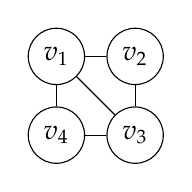
\begin{tikzpicture}
%\tikzstyle{place}=[circle,draw=blue!50,fill=blue!20,thick,inner sep=0pt,minimum size=6mm]
\begin{scope}[every node/.style={circle,draw}]           
    \node (A) at (2,2) {$v_1$};
    \node (B) at (3,2) {$v_2$};
    \node (C) at (3,1) {$v_3$};
    \node (D) at (2,1) {$v_4$};
    
    \path [-] (A) edge (B);
    \path [-] (A) edge (D);
    \path [-] (C) edge (D);
    \path [-] (C) edge (B);
    \path [-] (A) edge (C);
\end{scope}
\end{tikzpicture}
\caption{A chordal graph that comes from moralizing a non-singly connected DAG.}
\label{fg:chordal_over_4nodes}
\end{figure}

\begin{corollary}
Let $B_X$ be a set of Markov blankets over a variable set $X$. The problem of testing if $B_X$ is consistent with a polytree tree is in polynomial time.
\end{corollary}
\begin{proof}
Chordality can be verified in polynomial time \cite{tarjan1984simple}. \qed
\end{proof}

\textbf{Idea:} Since it is in polynomial time to check if a set of learned $B_X$ is consistent with a DAG or not, we could start the structure discovery process by learning a polytree over all variables in $X$. Then gradually build up a DAG from a polytree. In addition, because a polytree is a subset of DAGs, so there would be less number of consistent polytrees to a chordal graph than consistent DAGs to a WRS graph. 

\bibliographystyle{named}
\bibliography{/home/kl/Documents/causal_discovery_ref_list}

\end{document}